\chapter{Game AI}
\label{apdx:gameAI}

\section{Algorithms}

\begin{algorithm}
\caption{Negamax algorithm}
\label{alg:negamax}
\begin{algorithmic}
\Function{negamax}{depth}
    \If{$depth \leq 0$}
        \State \Return $value()$
    \EndIf
    \State $\alpha = -\infty$
    \ForAll{possible moves}
        \State $\alpha = max(\alpha, -negamax(depth-1))$
    \EndFor
    \State \Return $\alpha$
\EndFunction
\end{algorithmic}
\end{algorithm}

\section{``Gamers' survey'' in section~\ref{surveygamers} page~\pageref{surveygamers}}

\label{apdx:survey}
\subsection{Questions}

How good are you?
\begin{itemize}
    \item Very good
    \item Good
\end{itemize}


How important is the virtuosity? (to win the game)
reflexes, accuracy, speed, "mechanics"
\begin{itemize}
    \item 0 (not at all, or irrelevant)
    \item 1 (counts, can be game changing for people on equal level at other answers)
    \item 2 (counts a lot, can make a player win even if he is a little worse on lower importance gameplay features)
\end{itemize}


How important is deductive thinking? (to win the game)
"If I do A he can do B but not C" or "I see E so he has done D", also called analysis, forward inference."
\begin{itemize}
    \item 0 (not at all, or irrelevant)
    \item 1 (counts, can be game changing for people on equal level at other answers)
    \item 2 (counts a lot, can make a player win even if he is a little worse on lower importance gameplay features)
\end{itemize}


How important is inductive thinking? (to win the game)
"He does A so he may be thinking B" or "I see D and E so (in general) he should be going for F (learned)", also called generalization, "abstraction".
\begin{itemize}
    \item 0 (not at all, or irrelevant)
    \item 1 (counts, can be game changing for people on equal level at other answers)
    \item 2 (counts a lot, can make a player win even if he is a little worse on lower importance gameplay features)
\end{itemize}


How hard is decision-making? (to win the game)
"I have options A, B and C, with regard to everything I know about this game, I will play B (to win)", selection of a course of actions.
\begin{itemize}
    \item 0 (not at all, or irrelevant)
    \item 1 (counts, can be game changing for people on equal level at other answers)
    \item 2 (counts a lot, can make a player win even if he is a little worse on lower importance gameplay features)
\end{itemize}


You can predict the next move of your opponent:
(is knowledge of the game or of the opponent more important)
\begin{itemize}
    \item 1 by knowing what the best moves are / the best play for him?
    \item -1 by knowing him personally (psychology)?
    \item 0 both equal
\end{itemize}


What is more important:
\begin{itemize}
    \item 1 knowledge of the game (general strategies, tactics, timings)
    \item -1 knowledge of the map (specific strategies, tactics, timings)
    \item 0 both equal
\end{itemize}

\subsection{Results}

\begin{sidewaystable}

\begin{tabular}{|l|ccc|ccc|ccc|ccc|ccc|ccc|}
\hline
Game & \multicolumn{3}{|c|}{Virtuosity} & \multicolumn{3}{|c|}{Deduction} & \multicolumn{3}{|c|}{Induction} & \multicolumn{3}{|c|}{Decision-Making} & \multicolumn{3}{|c|}{Opponent} & \multicolumn{3}{|c|}{Knowledge}\\
 & \multicolumn{3}{|c|}{(sensory-motor)} & \multicolumn{3}{|c|}{(analysis)} & \multicolumn{3}{|c|}{(abstraction)} & \multicolumn{3}{|c|}{(acting)} & \multicolumn{3}{|c|}{-1: subjectivity} & \multicolumn{3}{|c|}{-1: map} \\
 & \multicolumn{3}{|c|}{[0-2]} & \multicolumn{3}{|c|}{[0-2]} & \multicolumn{3}{|c|}{[0-2]} & \multicolumn{3}{|c|}{[0-2]} & \multicolumn{3}{|c|}{1: objectivity} & \multicolumn{3}{|c|}{1: game} \\
 & top & rest & n & top & rest & n & top & rest & n & top & rest & n & top & rest & n & top & rest & n \\
\hline
Chess &  X & X & X  & 1.714 & 1.815 & 34 & 1.714 & 1.429 & 35 & 1.714 & 1.643 & 35 & 0.714 & 0.286 & 35 &  X & X & X  \\
Go &  X & X & X  & 2.000 & 1.667 & 16 & 2.000 & 1.600 & 16 & 2.000 & 1.600 & 16 & 1.000 & 0.533 & 16 &  X & X & X  \\
Poker &  X & X & X  & 1.667 & 0.938 & 22 & 1.667 & 1.562 & 22 & 1.333 & 1.625 & 22 & -0.167 & -0.375 & 22 &  X & X & X  \\
Racing & 2.000 & 1.750 & 19 & 0.286 & 0.250 & 19 & 0.571 & 0.000 & 19 & 1.286 & 0.833 & 19 & 0.571 & 0.455 & 18 & -0.286 & -0.333 & 19 \\
TeamFPS & 1.917 & 1.607 & 40 & 1.083 & 1.000 & 39 & 1.417 & 0.929 & 40 & 1.417 & 1.185 & 39 & 0.000 & 0.214 & 40 & -0.083 & -0.115 & 38 \\
FFPS & 2.000 & 2.000 & 22 & 1.250 & 1.000 & 21 & 1.125 & 1.077 & 21 & 1.125 & 1.231 & 21 & 0.250 & -0.154 & 21 & 0.250 & 0.083 & 20 \\
MMORPG & 1.118 & 1.000 & 29 & 1.235 & 0.833 & 29 & 1.176 & 1.000 & 29 & 1.235 & 1.250 & 29 & 0.471 & 0.250 & 29 & 0.706 & 0.833 & 29 \\
RTS & 1.941 & 1.692 & 86 & 1.912 & 1.808 & 86 & 1.706 & 1.673 & 83 & 1.882 & 1.769 & 86 & 0.118 & 0.288 & 86 & 0.412 & 0.481 & 86 \\
\hline
\end{tabular}
\label{fullsurveygamers}
\caption{Results of the survey (means) for ``top'' players and the ``rest'' of answers, along with the total number of answers (n).}
\end{sidewaystable}

%\chapter{Strategy}
%
%\section{Openings }
%NED stands for Not Enough Data\\
%Win rates of columns vs lines\\
%
%\begin{tabular}{|l|cccccc|}
%\hline
% & two gates & fast dt & speedzeal & reaver drop & corsair & nony\\
%\hline
%two gates &  0.5 & NED & NED & NED & NED & NED \\
%fast dt &  NED & 0.5 & NED & 0.454545454545 & NED & 0.445544554455 \\
%speedzeal &  NED & NED & NED & NED & NED & NED \\
%reaver drop &  NED & 0.545454545455 & NED & NED & NED & 0.608695652174 \\
%corsair &  NED & NED & NED & NED & NED & NED \\
%nony &  NED & 0.554455445545 & NED & 0.391304347826 & NED & 0.5 \\
%\hline
%\end{tabular}
%PvP Total Games: 296

%%% \begin{tabular}{|l|cccccc|}
%%% \hline
%%%  & two gates & fast dt & unknown & reaver drop & corsair & nony\\
%%% \hline
%%% bio &  NED & NED & NED & NED & NED & NED \\
%%% unknown &  NED & NED & 0.5 & NED & NED & NED \\
%%% drop &  NED & NED & NED & NED & NED & NED \\
%%% two facto &  NED & 0.552083333333 & NED & 0.477272727273 & NED & 0.578212290503 \\
%%% rax fe &  NED & 0.579439252336 & NED & 0.478260869565 & 0.363636363636 & 0.58371040724 \\
%%% vultures &  NED & NED & NED & NED & NED & NED \\
%%% \hline
%%% \end{tabular}
%%% PvT Total Games: 1657
 

%%% \begin{tabular}{|l|ccccccc|}
%%% \hline
%%%  & two gates & fast dt & unknown & speedzeal & reaver drop & corsair & nony\\
%%% \hline
%%% hydras &  NED & NED & NED & NED & NED & NED & NED \\
%%% unknown &  NED & NED & NED & NED & NED & NED & NED \\
%%% speedlings &  0.416666666667 & 0.75 & NED & NED & NED & NED & 0.5 \\
%%% lurkers &  NED & 0.492537313433 & NED & NED & NED & 0.444444444444 & 0.532981530343 \\
%%% fast mutas &  NED & 0.50641025641 & NED & NED & 0.5 & 0.526315789474 & 0.531590413943 \\
%%% \hline
%%% \end{tabular}
%%% PvZ Total Games: 1408


%\begin{tabular}{|l|cccccc|}
%\hline
% & bio & unknown & drop & two facto & rax fe & vultures\\
%\hline
%bio &  NED & NED & NED & NED & NED & NED \\
%unknown &  NED & NED & NED & NED & NED & NED \\
%drop &  NED & NED & NED & NED & NED & NED \\
%two facto &  NED & NED & NED & 0.5 & 0.517985611511 & NED \\
%rax fe &  NED & NED & NED & 0.482014388489 & 0.5 & NED \\
%vultures &  NED & NED & NED & NED & NED & NED \\
%\hline
%\end{tabular}
%TvT Total Games: 332
%
%\begin{tabular}{|l|cccc|}
%\hline
% & unknown & speedlings & lurkers & fast mutas\\
%\hline
%rax fe &  NED & NED & 0.546357615894 & 0.526315789474 \\
%drop &  NED & NED & NED & NED \\
%two facto &  NED & NED & NED & 0.379310344828 \\
%unknown &  0.5 & NED & NED & NED \\
%bio &  NED & NED & 0.5 & 0.7 \\
%\hline
%\end{tabular}
%TvZ Total Games: 1520
%
%
%\begin{tabular}{|l|cccc|}
%\hline
% & unknown & speedlings & lurkers & fast mutas\\
%\hline
%unknown &  NED & NED & NED & NED \\
%speedlings &  NED & 0.5 & NED & 0.388888888889 \\
%lurkers &  NED & NED & NED & NED \\
%fast mutas &  NED & 0.611111111111 & NED & 0.5 \\
%\hline
%\end{tabular}
%ZvZ Total Games: 148


\chapter{StarCraft AI}

\section{Datasets}
\label{appdx:datasets}

%\begin{tabular}{|l|c|c|c|c|c|c|}
%\end{tabular}
%
%\subsection{Ben Weber's dataset}
%     542 scmPvP_Protoss
%    1139 scmPvT_Protoss
%    1139 scmPvT_Terran
%    1024 scmPvZ_Protoss
%    1024 scmPvZ_Zerg
%     628 scmTvT_Terran
%    1150 scmTvZ_Terran
%    1150 scmTvZ_Zerg
%    1010 scmZvZ_Zerg
%
%
%\subsection{Our dataset}



\section{Algorithms}

\begin{algorithm}
\caption{(Simplified) Target selection heuristic, efficiently implemented with a enemy units $\leftrightarrow$ damages bidirectional map: $bimap : u, d \rightarrow (left : u \rightarrow d,\ right : d \rightarrow u)$}
\label{alg:targetselection}
\begin{algorithmic}
\Function{on\_death}{$unit$}
\State $remove\_incoming\_damages(unit.target, damages(unit,unit.target))$
\EndFunction

\Function{register\_target}{$unit, target$}
\State $add\_incoming\_damages(target, damages(unit, target))$
\State $unit.target \leftarrow target$
\EndFunction

\Function{select\_target}{$unit$}
\ForAll{$eunit \in focus\_fire\_order(enemy\_units)$}
    \If{$eunit.type \in priority\_targets(unit.type)$}
        \If{$in\_range(unit, eunit)$}
            \State $register\_target(unit, eunit)$
        \ElsIf{$unit.prio\_target ==$ NULL}
            \State $unit.prio\_target \leftarrow eunit$
        \EndIf 
    \EndIf 
\EndFor
\If{$unit.target ==$ NULL}
    \ForAll{$eunit \in focus\_fire\_order(enemy\_units)$}
        \If{$in\_range(unit, eunit)$}
            \State $register\_target(unit, eunit)$
        \EndIf 
    \EndFor
\EndIf
\If{$unit.target ==$ NULL \textbf{and} $unit.prio\_target ==$ NULL} %%% TODO formatting
    $unit.prio\_target \leftarrow closer(unit, enemy\_units)$
\EndIf
\EndFunction
\end{algorithmic}
\end{algorithm}

\begin{algorithm}
\caption{Flow algorithm making sure there are no convex closures}
\label{alg:flood}
\begin{algorithmic}
\Function{init}{$region$}
    %\State $\{Flow_{i,j} \leftarrow -1 | Flow_{i,j} \in region\}$
    %\State $\{Dir_{i,j} \leftarrow (0,0) | Dir_{i,j} \in region\}$
    \State $\{dir_{i,j} \leftarrow list() | (i,j) \in region\}$
    \State $updated \leftarrow \{(i,j) | (i,j) \in entrance(region)\}$
    %\State $\{Flow_{i,j} \leftarrow 1 | (i,j) \in Updated\}$
    \State $\{dir_{i,j} \leftarrow dir\_towards(region) | (i,j) \in updated\}$
    %\While{$(\exists Flow_{i,j} == -1) \ \mathrm{or}\ (\exists Dir_{i,j} == (0,0))$}
    \While{$\exists dir_{i,j} == list()$}
        \State $(sources,new\_updated) \leftarrow neighbours\_couples(updated)$
        \ForAll{$((x,y),(i,j)) \in (sources,new\_updated)$}
            %\If{$(i-x,j-y) \neq Dir_{x,y}$}
            \If{$(x-i,y-j) \notin dir_{x,y}$}
                \State $dir_{i,j}.append((i-x, j-y))$
            %    \State $Flow_{i,j} += 1$
            \EndIf
        \EndFor
        \State $updated \leftarrow new\_updated$
    \EndWhile
\EndFunction

\Function{build}{$i,j$}
\ForAll{$(x,y) \in neighbours(i,j)$}
    \State $dir_{x,y}.remove((x-i, y-j))$
    \If{$dir_{x,y}.empty()$}
        \State $build(x,y)$
    \EndIf
\EndFor
\EndFunction
\end{algorithmic}
\end{algorithm}

\begin{algorithm}
\caption{Production/Construction Planning}
\label{alg:planning}
\begin{algorithmic}
\Function{init}{}
\EndFunction
\end{algorithmic}
\end{algorithm}

\section{Figures}
\begin{figure}[ht]
\begin{center}
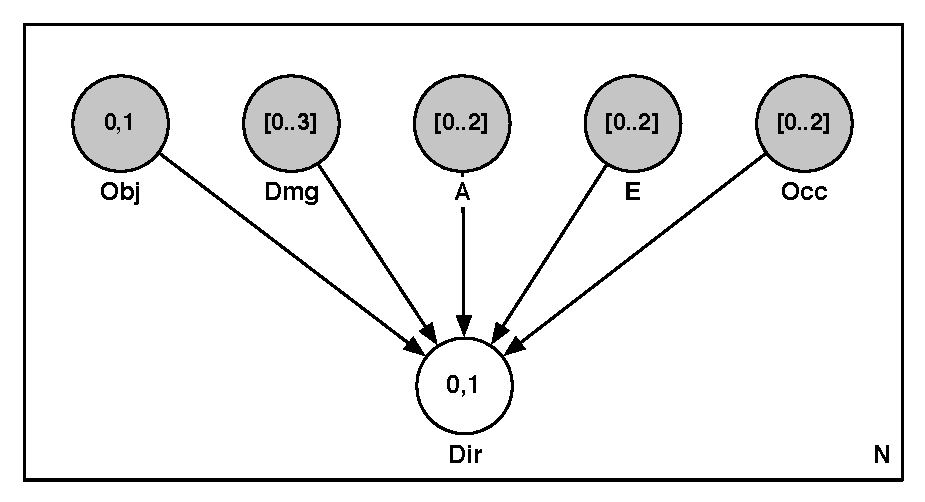
\includegraphics[width=8cm]{images/BayesianUnit_plate.pdf}
\caption{Plate diagram of a Bayesian unit with $N$ possible directions.}
\label{fig:BayesianUnit_plate}
\end{center}
\end{figure}

\begin{figure}[ht]
\begin{center}
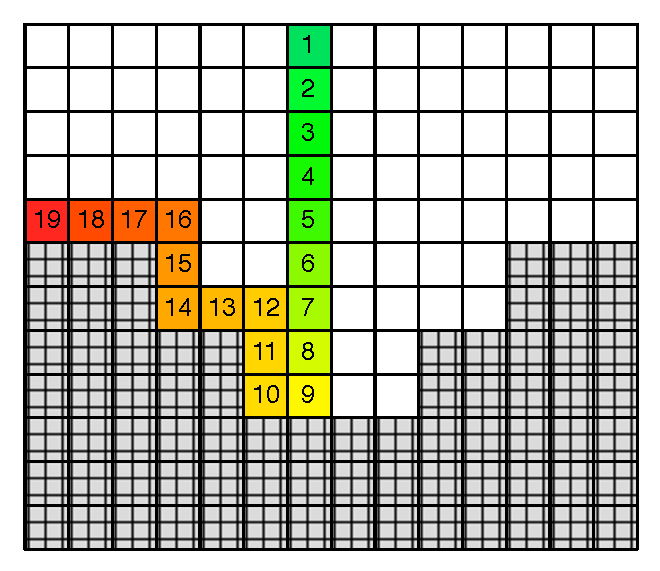
\includegraphics[width=8cm]{images/trailing_pheromones.pdf}
\caption{Example of trailing repulsive charges (repulsive ``pheromones'') at already visited positions for Bayesian units to avoid being blocked by local optimums. The trajectory is indicated by the increasing numbers (most recent unit position in 19) and the (decaying) strength of the trailing repulsion is weaker in green and stronger in red. Related to \ref{BayesianUnitCCL}.}
\label{fig:BayesianTrailingPheromone}
\end{center}
\end{figure}

\begin{figure}[ht]
\begin{center}
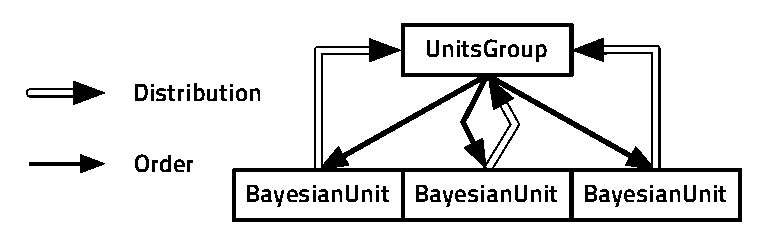
\includegraphics[width=8cm]{images/UnitsGroup_BayesianUnits.pdf}
\caption{Example of the decision taken at the units group level from ``compressed'' information in the form of the distribution on $Dir$ for each Bayesian unit. This can be viewed as a simple optimization problem (maximize sum of probabilities of decisions taken) or as a constraint satisfaction problem (CSP) like ``no unit should be left behind/die/dissatisfied''. Related to \ref{BayesianUnitCCL}}
\label{fig:BayesianUnitsGroup}
\end{center}
\end{figure}


\begin{figure}[ht]
\begin{center}
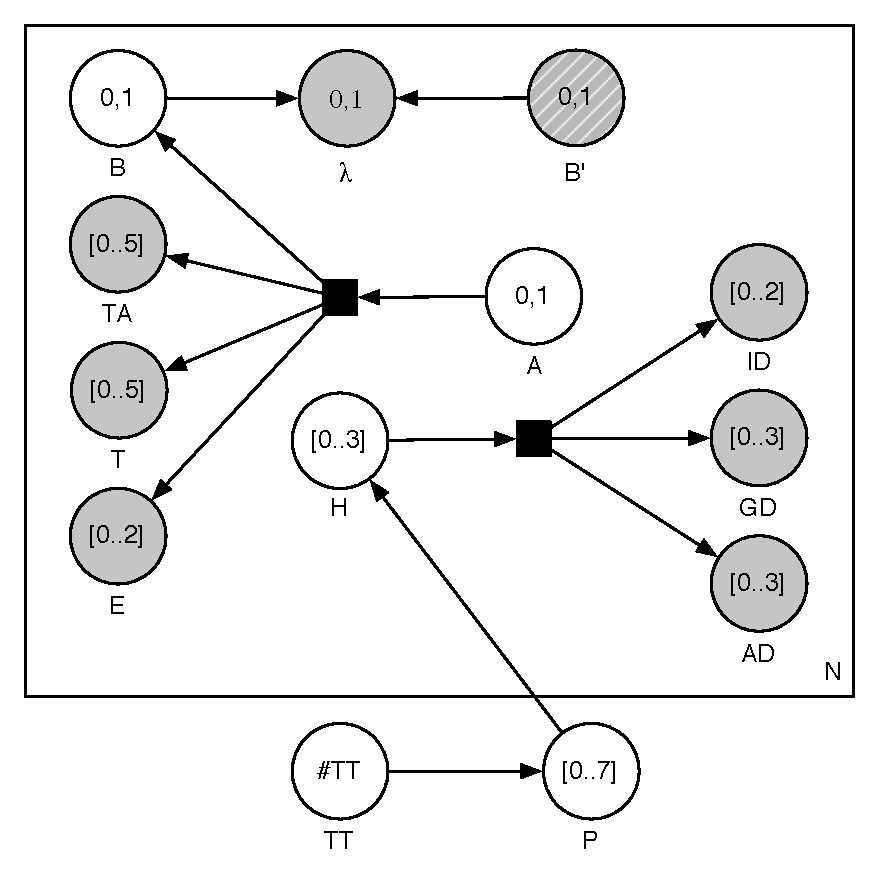
\includegraphics[width=8cm]{images/SpecialTactics_plate.pdf}
\caption{Plate diagram of the Bayesian tactical model in prediction (we know $ID, AD, GD$)}
\label{fig:SpecialTactics_plate}
\end{center}
\end{figure}

